\documentclass{article}%
\usepackage[T1]{fontenc}%
\usepackage[utf8]{inputenc}%
\usepackage{lmodern}%
\usepackage{textcomp}%
\usepackage{lastpage}%
\usepackage[head=40pt,margin=0.5in,bottom=0.6in]{geometry}%
\usepackage{graphicx}%
%
\title{\textbf{La sanidad de Brasil descarta que glifosato sea cancerígeno}}%
\author{AFP}%
\date{04/03/2019}%
%
\begin{document}%
\normalsize%
\maketitle%
\textbf{URL: }%
http://www.eluniversal.com/estilo{-}de{-}vida/34385/la{-}sanidad{-}de{-}brasil{-}descarta{-}que{-}glifosato{-}sea{-}cancerigeno\newline%
%
\textbf{Periodico: }%
EU, %
ID: %
34385, %
Seccion: %
estilo{-}de{-}vida\newline%
%
\textbf{Palabras Claves: }%
NO\_TIENE\newline%
%
\textbf{Derecho: }%
2.1%
, Otros Derechos: %
\newline%
%
\textbf{\textit{Anvisa aprobó que el estudio sea sometido a consulta pública durante 90 días}}%
\newline%
\newline%
%
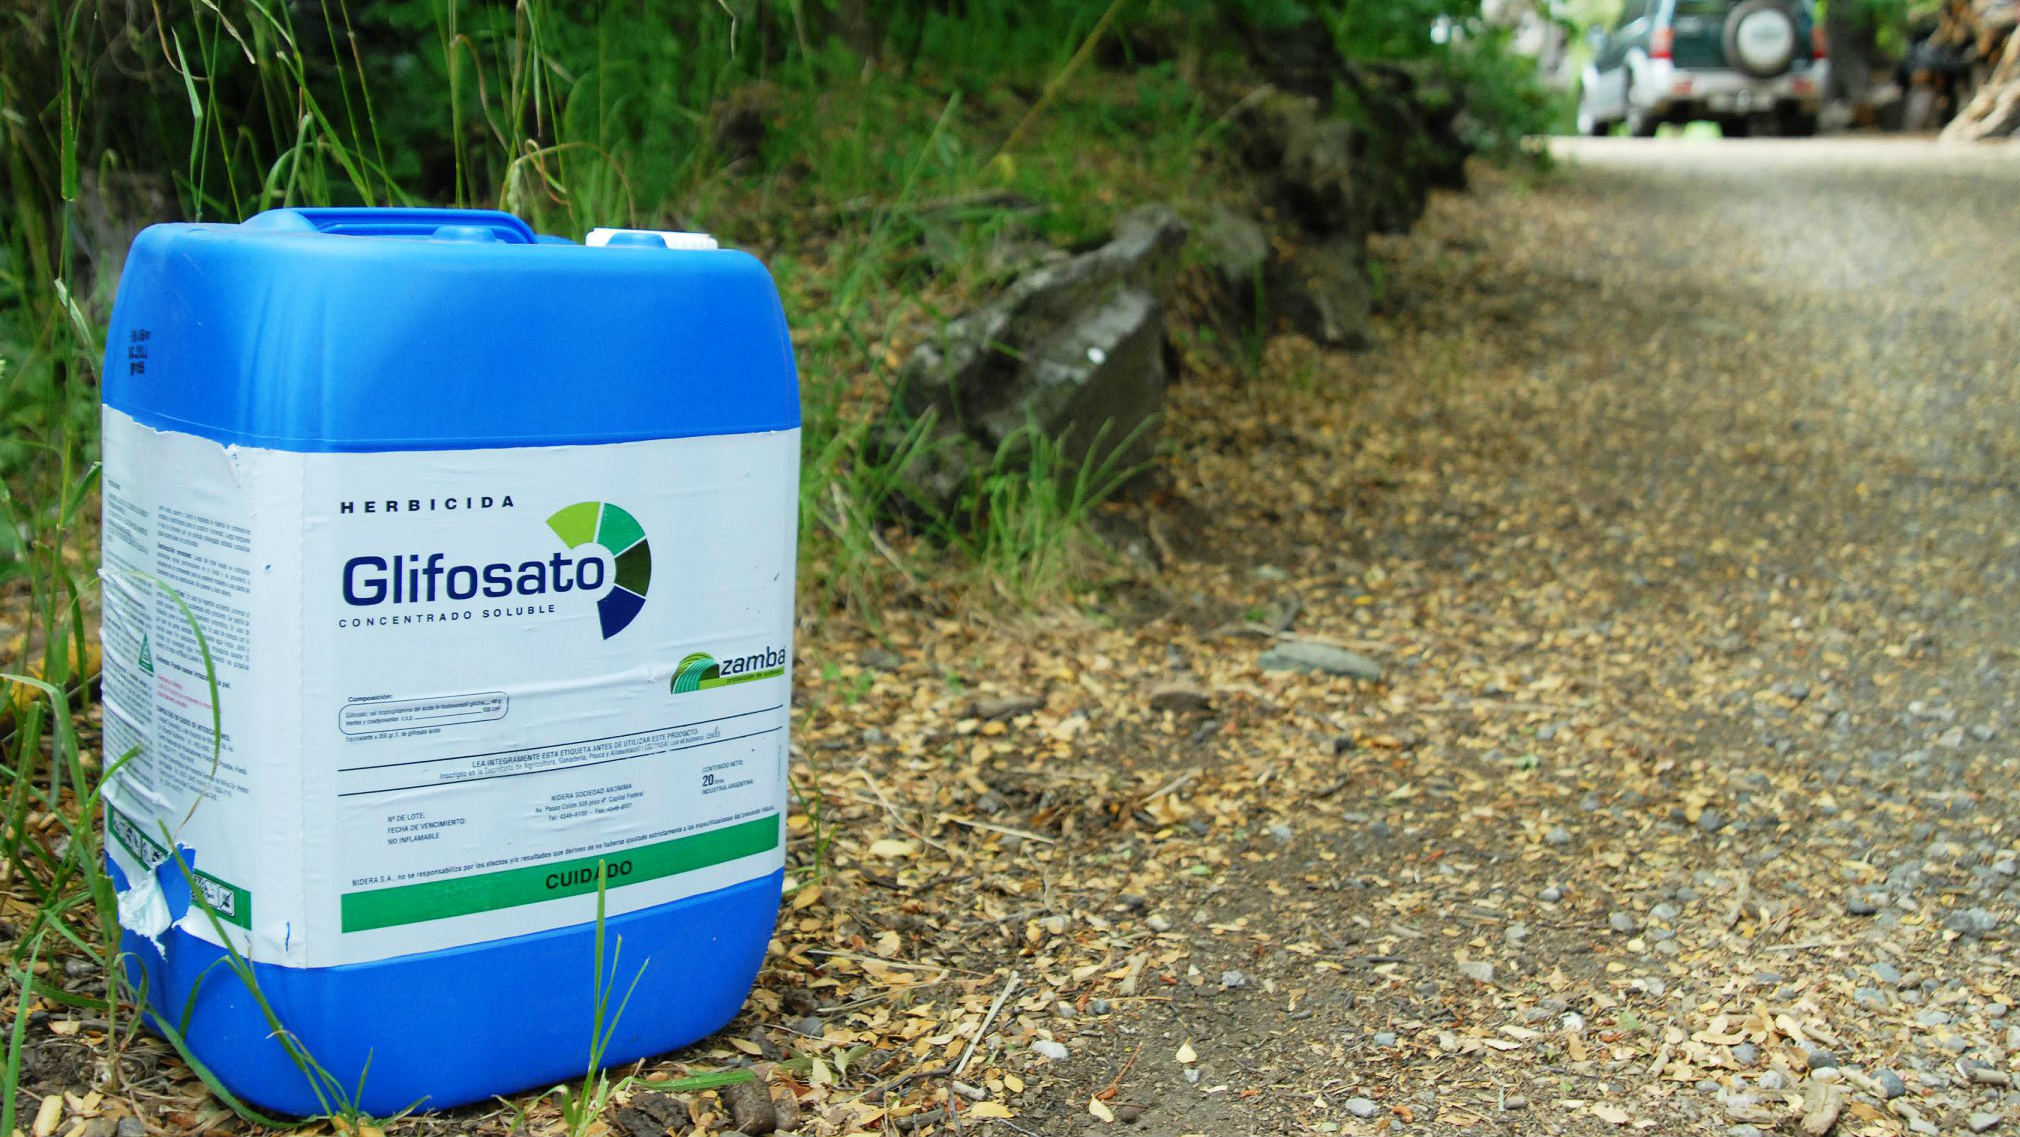
\includegraphics[width=300px]{EU_34385.jpg}%
\newline%
%
Un estudio de la autoridad sanitaria de Brasil, Anvisa, determinó que el glifosato no es cancerígeno, pero recomendó algunas medidas de precaución para continuar su amplio uso en la producción agrícola del gigante sudamericano, informó el martes una fuente del organismo.%
\newline%
%
"En nuestra evaluación concluimos que no hay pruebas suficientes para considerar el glifosato como cancerígeno", dijo a la AFP Adriana Pottier, gerente de monitoreo y evaluación de riesgo de la Agencia Nacional de Vigilancia Sanitaria (Anvisa).%
\newline%
%
El glifosato, considerado desde 2015 por la Organización Mundial de la Salud (OMS) como "cancerígeno probable", es un producto utilizado en los cultivos de cereales y oleaginosas de Brasil, segundo productor mundial de soja y maíz.%
\newline%
%
Pottier explicó que los riesgos que implica el uso del producto, conocido comercialmente como RoundUp, demandaron algunas medidas de precaución para proteger a los trabajadores que están en contacto con el uso de glifosato y para los consumidores.%
\newline%
%
Por ejemplo, dice Pottier, se recomendó la utilización de tecnologías que reduzcan la aspersión del glifosato; que la aplicación, mezcla y abastecimiento de la sustancia sean realizadas por diferentes personas, y que después de la fumigación de un campo se prohíba el ingreso de los trabajadores por un tiempo prudencial.%
\newline%
%
Este martes Anvisa aprobó que el estudio sea sometido a consulta pública durante 90 días; luego de ese periodo el organismo evaluará los aportes recibidos y para finales de 2019 se espera que concluya el proceso de "reevaluación toxicológica" del glifosato "con la publicación de un reglamento sobre el tema", detalló Pottier.%
\newline%
%
La responsable destacó que la conclusión del equipo de Anvisa es coherente con las realizadas por organismos internacionales como la Agencia Europea de Sustancias y Mezclas Químicas (ECHA) y la agencia estadounidense de protección del medioambiente (EPA).%
\newline%
%
El RoundUp es propiedad del gigante químico y farmacéutico alemán Bayer, tras haberlo comprado a la estadounidense Monsanto el año pasado.%
\newline%
%
El glifosato, elogiado por los agricultores por su eficiencia y bajo costo, está bajo la lupa en Europa, particularmente en Francia, donde las autoridades prohibieron en enero un tipo de herbicida, el Roundup Pro 360.%
\newline%
%
En noviembre de 2017, la Unión Europea (UE) renovó la homologación del glifosato por un período de cinco años, pero el presidente francés Emmanuel Macron se comprometió a prohibirlo antes de 2021.%
\newline%
%
\end{document}